\documentclass[10pt]{article}

% Lines beginning with the percent sign are comments
% This file has been commented to help you understand more about LaTeX

% DO NOT EDIT THE LINES BETWEEN THE TWO LONG HORIZONTAL LINES

%---------------------------------------------------------------------------------------------------------

% Packages add extra functionality.
\usepackage{
	times,
	graphicx,
	epstopdf,
	fancyhdr,
	amsfonts,
	amsthm,
	amsmath,
	algorithm,
	algorithmic,
	xspace,
	hyperref,
        qtree}
\usepackage[left=1in,top=1in,right=1in,bottom=1in]{geometry}
\usepackage{sect sty}	%For centering section headings
\usepackage{enumerate}	%Allows more labeling options for enumerate environments 
\usepackage{epsfig}
\usepackage[space]{grffile}
\usepackage{booktabs}
\usepackage{amsmath}
\usepackage[super]{nth}

% This will set LaTeX to look for figures in the same directory as the .tex file
\graphicspath{.} % The dot means current directory.

\pagestyle{fancy}

\lhead{\YOURID}
\chead{\projectName: Language Specification}
\rhead{\today}
\lfoot{CSCI 334: Principles of Programming Languages}
\cfoot{\thepage}
\rfoot{Spring 2020}

% Some commands for changing header and footer format
\renewcommand{\headrulewidth}{0.4pt}
\renewcommand{\headwidth}{\textwidth}
\renewcommand{\footrulewidth}{0.4pt}

% These let you use common environments
\newtheorem{claim}{Claim}
\newtheorem{definition}{Definition}
\newtheorem{theorem}{Theorem}
\newtheorem{lemma}{Lemma}
\newtheorem{observation}{Observation}
\newtheorem{question}{Question}

\setlength{\parindent}{0cm}
%---------------------------------------------------------------------------------------------------------

% DON'T CHANGE ANYTHING ABOVE HERE

% Edit below as instructed
\newcommand{\YOURID}{Petros Markopoulos}	% Replace "Your Name Here" with your name
\newcommand{\projectName}{\textbf{FUNny }}
\newcommand{\langName}{\textbf{FUNny Language }}
\newcommand{\intName}{\textbf{FUNny Visual Interface }}
\newcommand{\ProblemHeader}	% Don't change this!

\begin{document}

\vspace{\baselineskip}	% Add some vertical space

% Refer to the lab handouts to determine what should go in each of these sections.  Each lab is additive.  So lab 8 should include everything you wrote in lab 7.  Lab 9 should include everything you wrote in lab 8, etc.

\section{Introduction}
In this course we have spent a decent chunk of our time looking at the advantages of functional programming. We first discussed LISP and the innovations it brought, then we looked at the reading "Why Functional Programming Matters", which gave a detailed account of some benefits of functional programming and now we are learning F\#. It is safe to say, then, that functional programming is the unofficial theme of this course. But, if functional programming is so useful, why was it unfamiliar to most of us before this class? Why is it regarded as something complex and scary when it is neither, when, in fact, at its core it is very simple and elegant? In my view it is because it is because it is not introduced early in a programmer's life and so, when the time comes for one to learn it, they are already familiar with other common programming paradigms and they have a hard time adapting to the new way of thinking and coding.\\\\
This is the problem that my project, tentatively named \projectName, is aiming to solve. \projectName\ will consist of a simple functional programming language, and a visual programming environment for that language. The visual environment will work based on the simple view of functions as machines that transform the input given to them into output, just like we have seen multiple times in class. The programmer will have some pre-built machines at their disposal and the ability to compose them by piping their outputs to other machines in order to create more complex machines. \projectName\ is aimed mainly to children as an introduction to functional programming. It's goal is to demystify functional programming, illustrate the simplicity of its core concepts in a fun, enjoyable way and facilitate its learning, just like visual programming environments like Scratch are helpful as introductions to the imperative paradigm.


\section{Design Principles}
From now on, \projectName  will be used to refer to the project as a whole. The language will be refered to as \langName and the interface as \intName.\\\\
Naturally, \langName will be a simple functional programming language. It will be based on the idea of pure functions and declarative statements. My aim is for the code to be highly readable and descriptive, so as to facilitate the understanding of the code and its correlation with the \intName by younger children who may have a hard time reading sybmolic expressions. Since the \langName is not meant to be written, but rather generated using the \intName, it can be very strict in its form (the use of whitespace for example), since automatically generating consistent code is fairly simple.\\\\
\intName will be a visual interface utilizing the analogy between functions and machines that convert input into output. What will guide the implementation of the \intName will be the design of the \langName, as I would like them to feel strongly correlated, and also its design highly depends on the features that end up being implemented in the language. Aesthetically speaking, the \intName will be minimalistic, not only because I find that style to be pleasing, but also because I lack the ability to create any more intricate design.


\clearpage
\section{Example Programs}
\begin{enumerate}
    \item
        \[
            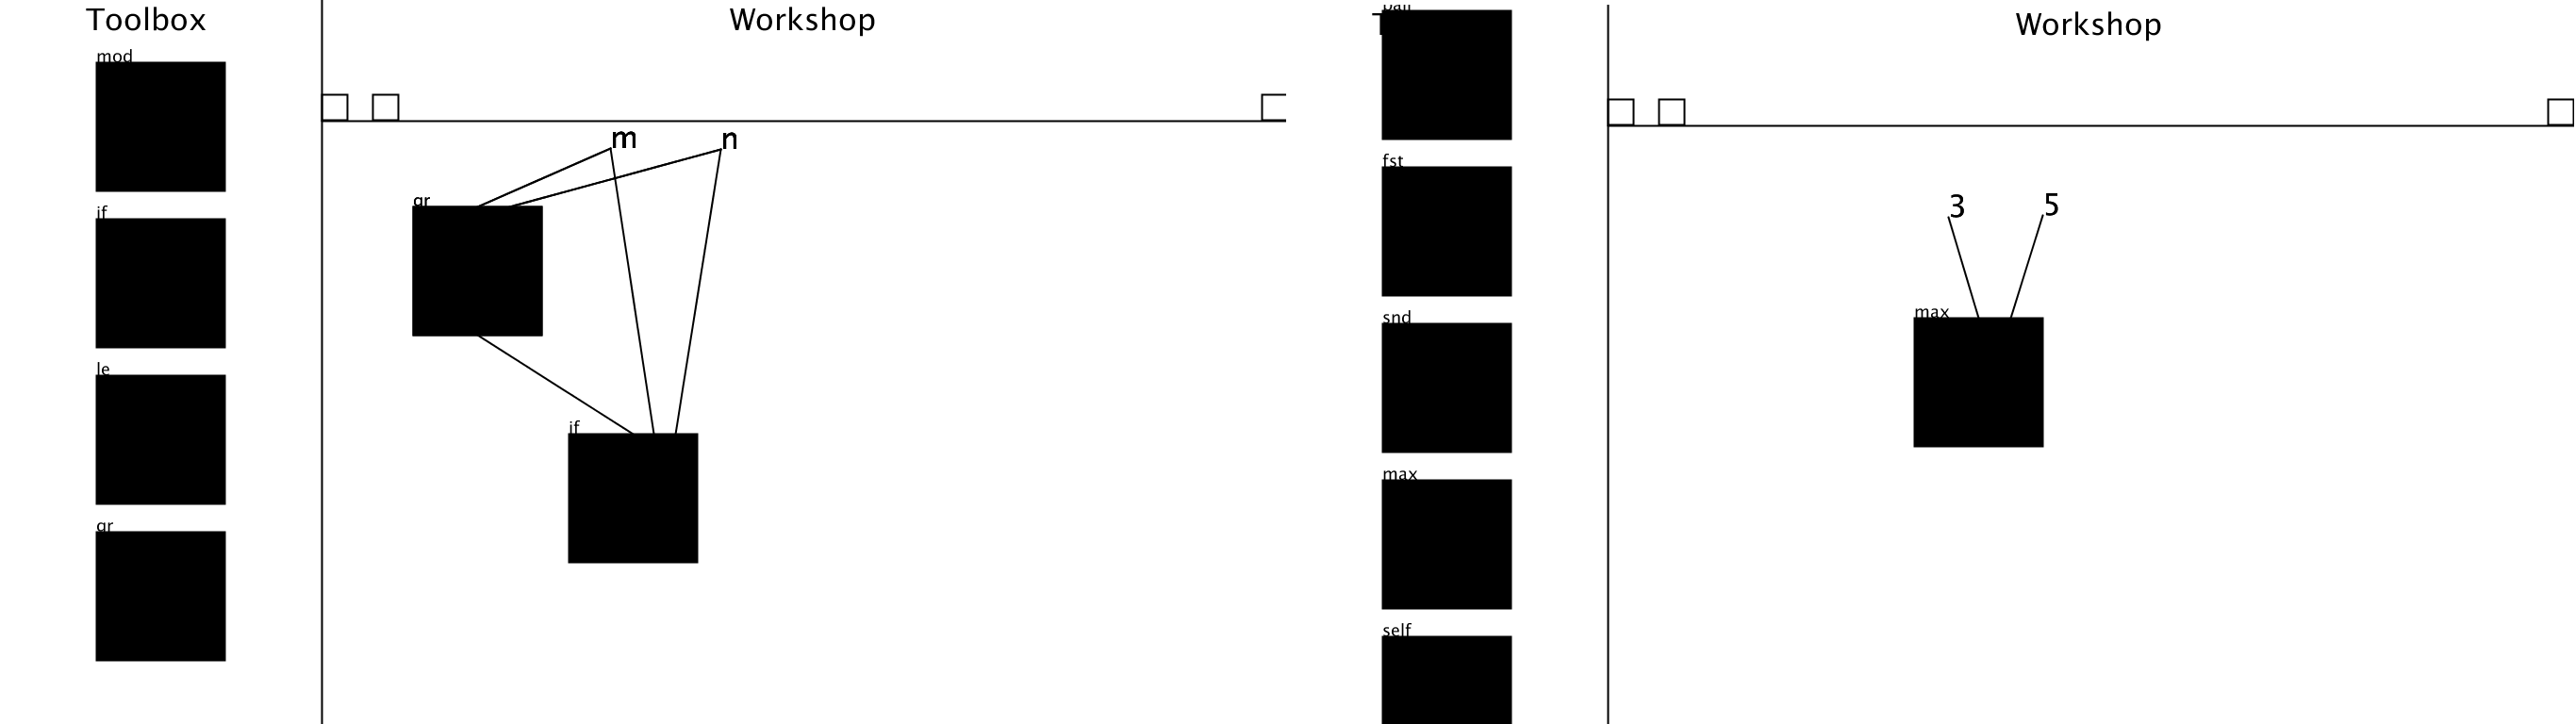
\includegraphics[width=\textwidth]{funny_program_example_1_visual_complete.png}
        \]
            In the left picture above, a new function is defined, which finds the maximum of two numbers. And in the right one, it is called with the arguments 3 and 5.\\
        The text of the program that the above generates is
        \[
            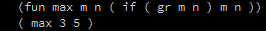
\includegraphics[width=\textwidth]{funny_program_example_1_text.png}
        \]
    \item
        \[
            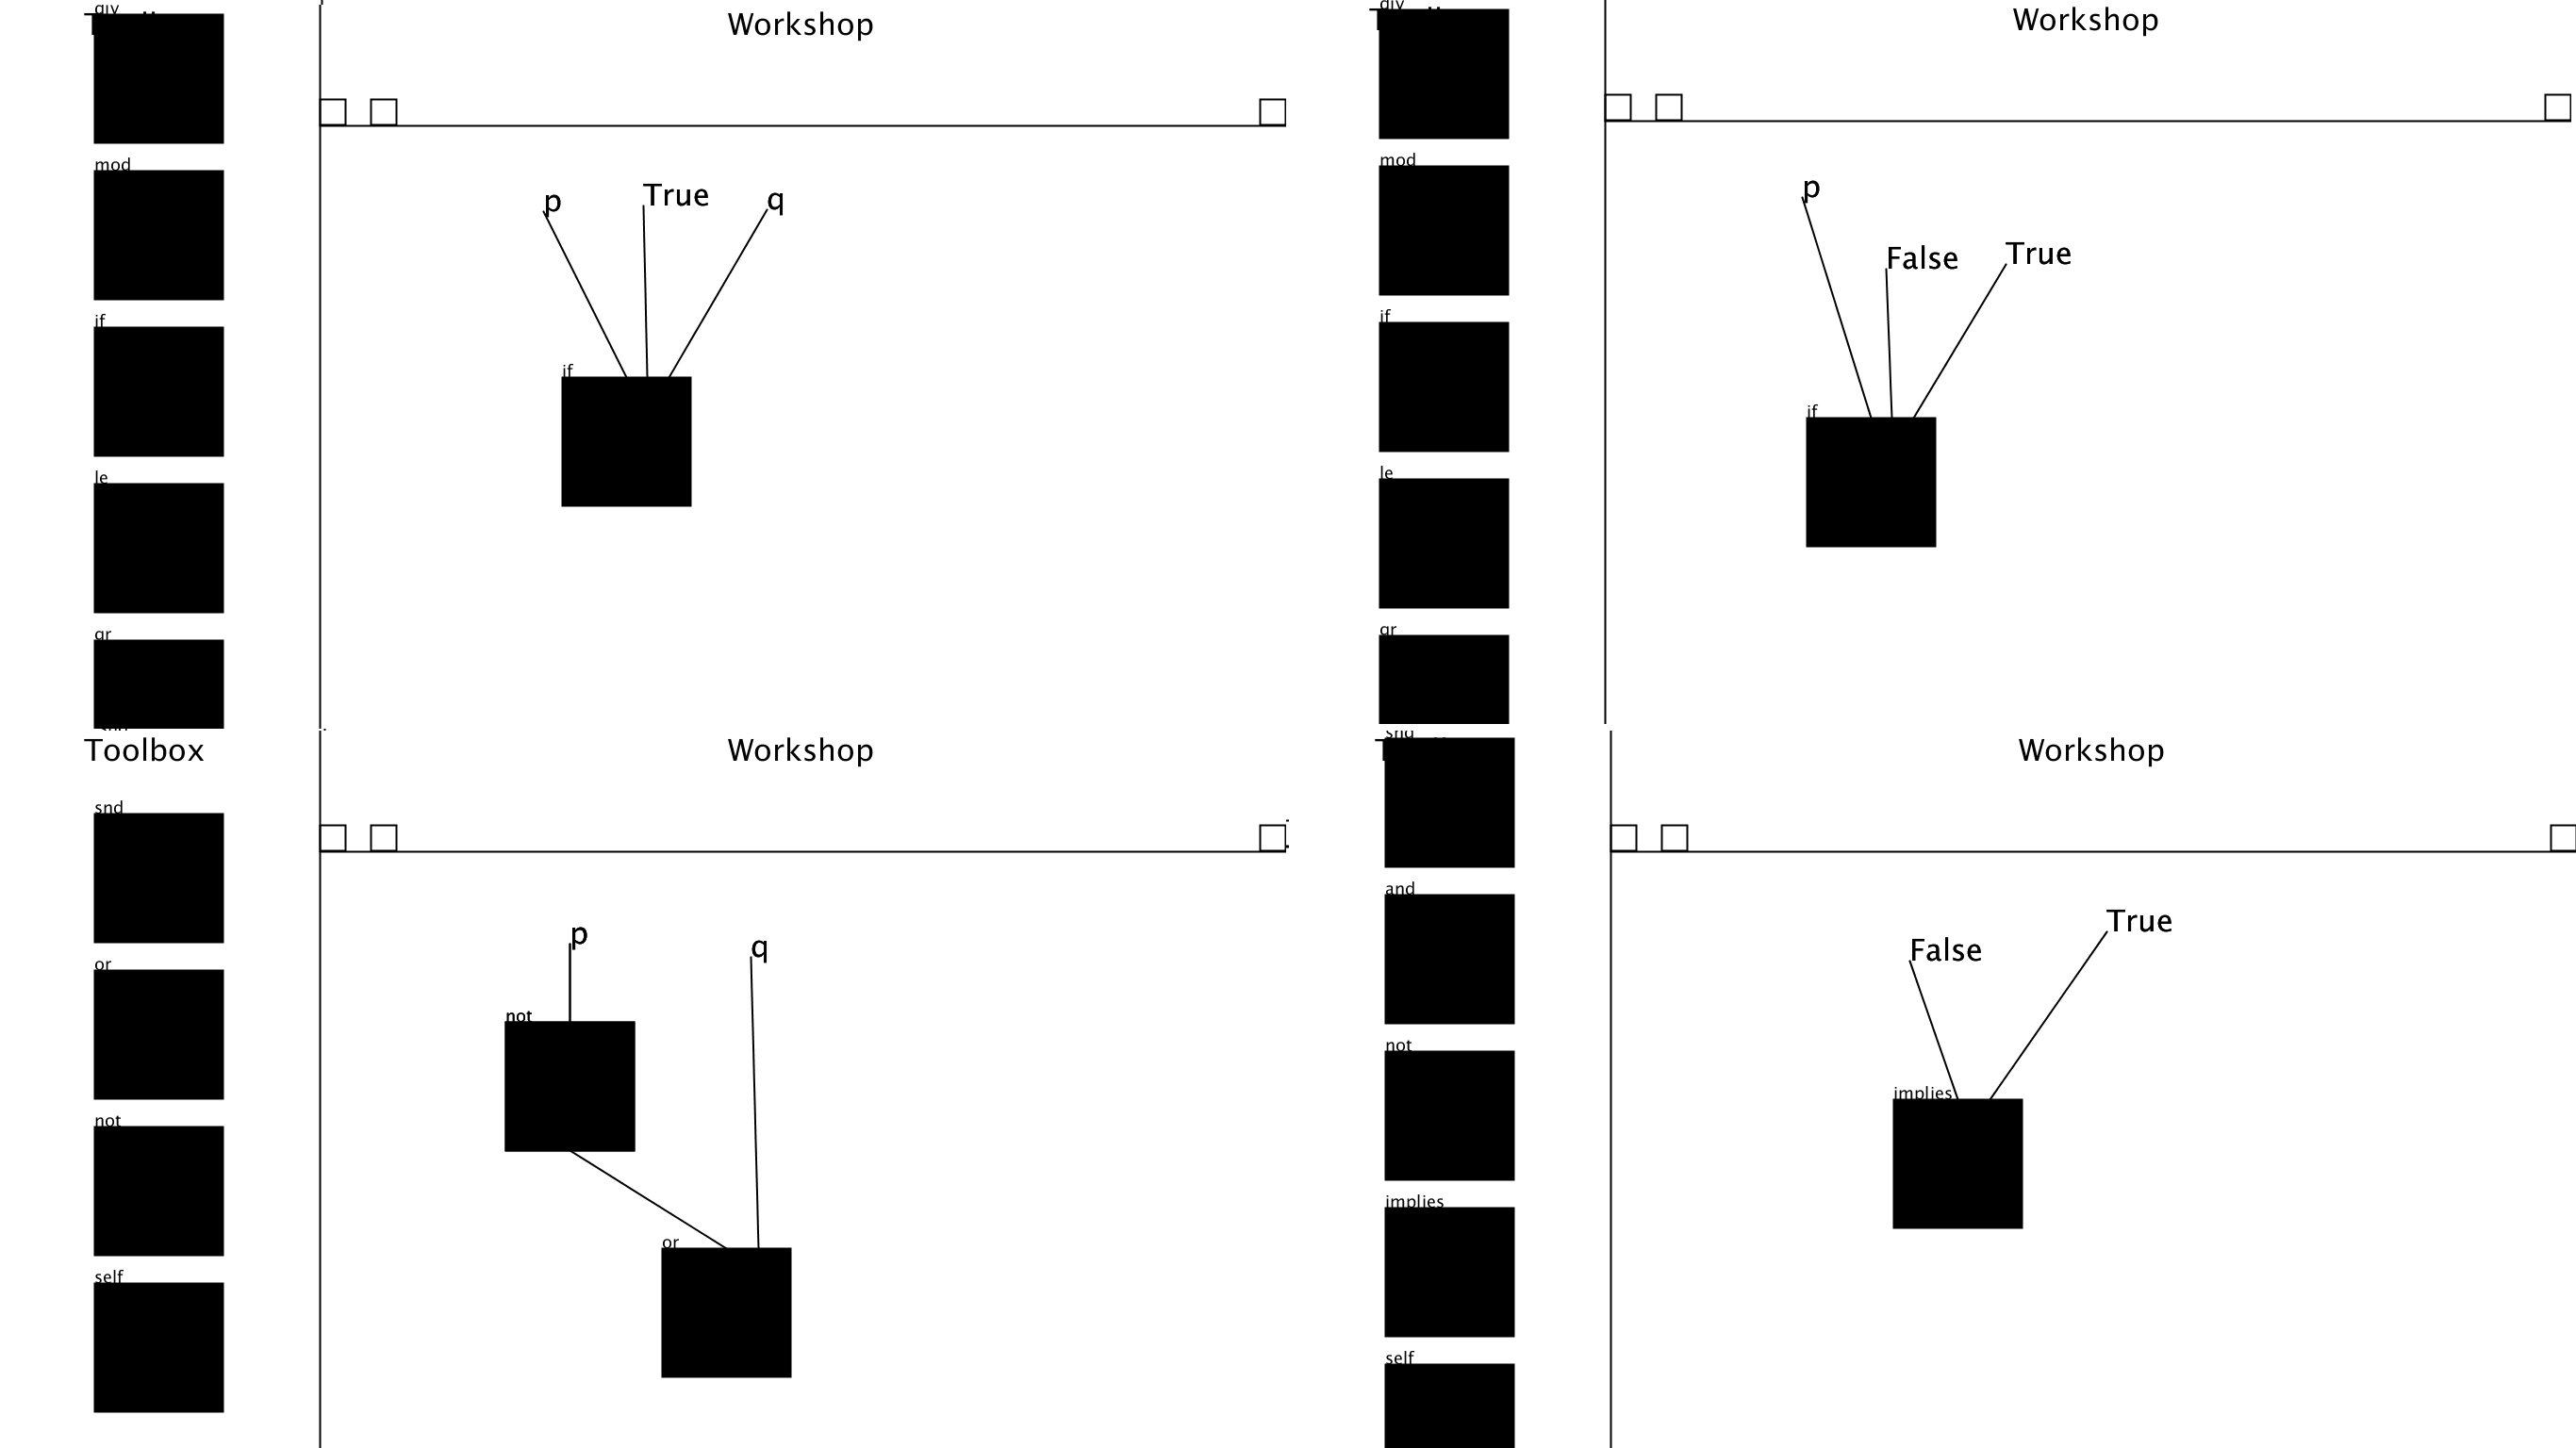
\includegraphics[width=\textwidth]{funny_program_example_2_visual_complete.png}
        \]
            In the top two picture above, some new functions is defined: the boolean operators \emph{or, not}. In the lower-left one, they are combined to define the function \emph{implies} which calculates the matching logic operator for two values. Then \emph{implies} is called with the arguments False and True.\\
        The text of the program that the above generates is
        \[
            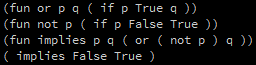
\includegraphics[width=\textwidth]{funny_program_example_2_text.png}
        \]
    \item
        \[
            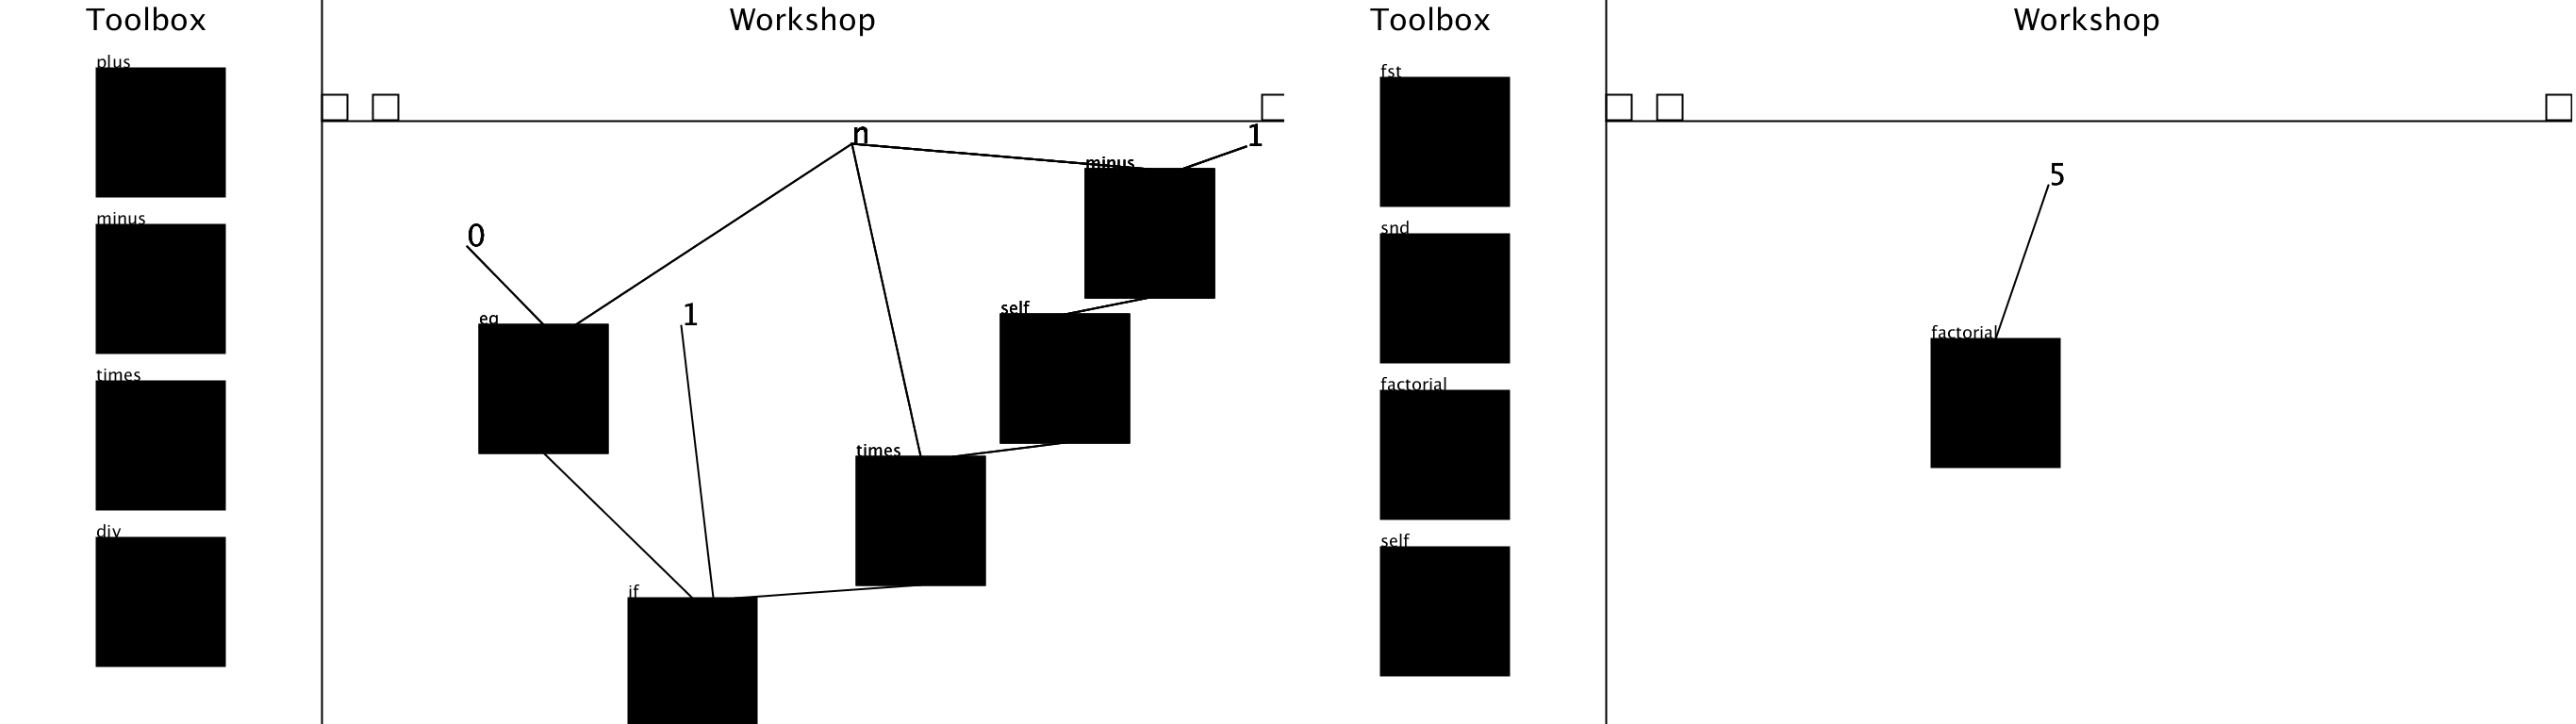
\includegraphics[width=\textwidth]{funny_program_example_3_visual_complete.png}
        \]
            In the left picture above, a new function is defined, which finds the factorial of a number. And in the right one, it is called with the argument 5.\\
        The text of the program that the above generates is
        \[
            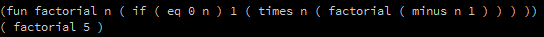
\includegraphics[width=\textwidth]{funny_program_example_3_text.png}
        \]
\end{enumerate}


\section{Language Concepts}
The core concept of the \langName is functions. Currently the \langName supports of functions of integers, booleans and pairs. They are always pure functions, meaning that their only effect when given an input is to produce an output. There is no mutable data in \langName and so variables don't play an important role, except for passing arguments to functions. Recursion is also a very important concept as it is in any functional programming language, since it is the sole way of implementing complex functionality and it is also supported in the current version of the language.

\clearpage
\section{Syntax}
The current grammar for the language is the following:
\begin{verbatim}
<expression> ::=
             |<sequence>
             |<value>
             |<application>
             |<fundefinition>
<sequence> ::= 
           |<value>
           |<application>
           |(<fundefinition>, <sequence>)
<value> ::= <primitive>
<application> ::= <word> <expression>+
<fundefinition> ::= <word> <word>+ <expression> 
<primitive> ::=
            |<bool>
            |Nil
            |<number>
            |<pair>
            |<arg>
<bool> ::= True | False
<number> ::= <d><number> | <d>
<d> ::= 0 | 1 | 2 | 3 | 4 | 5 | 6 | 7 | 8 | 9
<pair> ::= [<primitive>, <primitive>]
<arg> ::= <word>
<word> ::= <l><word> | <l>
<l> ::= a | b | c | d | e | f | g | h | i | j | k | l | m | n | o | p | q | r | s | t | u
      | v | w | x | y | z
      | A | B | C | D | E | F | G | H | I | J | K | L | M | N | O | P | Q | R | S | T | U
      | V | W | X | Y | Z
\end{verbatim}
To understand the syntax better let's look at the ASTs generated from the example programs:
\begin{enumerate}
    \item
        \begin{center}
            \Tree [.{SEQUENCE} [.{FUNDEFINITION} {max} [.{LIST} {m} {n} ] [.{APPLICATION} {if} [.{LIST} [.{APPLICATION} {gr} {m} {n} ] {m} {n} ] ] ] [.{APPLICATION} {max} [.{LIST} {3} {5} ] ] ]
        \end{center}
        \clearpage
    \item
        \begin{center}
            \resizebox{0.9\textwidth}{!}{%
                \Tree [.{SEQUENCE} [.{FUNDEFINITION} {or} [.{LIST} {p} {q} ] [.{APPLICATION} {if} [.{LIST} {p} {True} {q} ] ] ] [.{SEQUENCE} [.{FUNDEFINITION} {not} {p} [.{APPLICATION} {if} [.{LIST} {p} {False} {True} ] ] ] [.{SEQUENCE} [.{FUNDEFINITION} {implies} [.{LIST} {p} {q} ] [.{APPLICATION} {or} [.{LIST} [.{APPLICATION} {not} {p} ] {q} ] ] ] [.{APPLICATION} {implies} {False} {True} ] ] ] ]
            }
        \end{center}
    \item
        \begin{center}
            \resizebox{0.9\textwidth}{!}{%
                \Tree [.{SEQUENCE} [.{FUNDEFINITION} {factorial} {n} [.{APPLICATION} {if} [.{LIST} [.{APPLICATION} {eq} [.{LIST} {0} {n} ] ] {1} [.{APPLICATION} {times} [.{LIST} {n} [.{APPLICATION} {factorial} [.{APPLICATION} {minus} [.{LIST} {n} 1 ] ] ] ] ] ] ] ] [.{APPLICATION} {factorial} {5} ] ]
            }
        \end{center}
\end{enumerate}
For the \intName, the "syntax" is fairly intuitive. Taking a "machine" from the toolbox to the workspace allows the programmer to connect inputs to it by first clicking on the input and then on the machine, and connect its output to different machines by clicking on it and then clicking on the other machine.

\section{Semantics}
\begin{tabular}{|p{2cm} | p{4cm} | p{10cm}|}
    \hline
    \textbf{Syntax} & \textbf{Abstract Syntax} & \textbf{Meaning} \\
    \hline
    n & Value (Number of int) & A primitive value holding an integer. It is stored as an F\# integer.\\
    \hline
    True & Value (Boolean True) & A primitive value: holds the boolean value true.\\
    \hline
    False & Value (Boolean False) & A primitive value: holds the boolean value false.\\
    \hline
    Nil & Value Nil & A primitive value: holds the value nil (which can stand in for things line an empty list)\\
    \hline
    word & Value (Arg of string) & A primitive value: holds the name of the argument of a function. It is only meant to be used as part of function definitions.\\
    \hline
    ( name a1 a2 ... an ) & Application name [a1; a2; ...; an] & Application of arguments a1, a2, ..., an to the function `name`\\
    \hline
    (fun name a1 ... an exp) & FunctionDefinition name [a1;...;an] exp & Define the word `name` to correspond to the expression `exp` substituting values for a1, ..., an.\\
    \hline
    exp1\newline exp2 & Sequence (exp1, exp2) & Sequential evaluation of exp1, exp2. exp1 has to be a function definition.\\
    \hline
\end{tabular}
\\
Types in the \langName are checked at runtime. All expressions are parenthesized so there is no need to define precedence and associativity.\\
As for the semantics of the GUI, I will try to desribe them here:\\
A line connecting a primitive to function means that that primitive is being passed as an argument to that function. The arguments are passed to functions from left to right (meaning that the first argument is the one whose line connects farther to the right than all the other arguments, the second is the next one, etc).\\
For functions, lines coming in on the top are the arguments and a single line coming out of the bottom of the box is the output.\\
Any input that is not a number or "True", "False" or "Nil" is interpreted as an argument, and the function being built is interpreted as a function definition and not as a function application. Those arguments can be passed around as values and they will be substituted with concrete values upon applying the function.\\
Recursion is supported through the use of the self function. The self function is available in the toolbox and should only be used in function definitions, not applications. It stands in for the function being built as a whole and produces the appropriate code when it is run. It works like any other function, taking in inputs and producing an output.\\

\section{Remaining Work}
I want to work on adding real numbers in the \langName and higher order functions, since those two would allow for much more interesting programs. Especially for higher order functions it will be quite the challenge, so I don't know whether these features will make it into the project.\\
Other than that I want to improve the appearance and usability of the \intName because at it's current form it is very hard to use and understand.

% DO NOT DELETE ANYTHING BELOW THIS LINE
\end{document}
